\documentclass[12pt]{article}
\usepackage[utf8]{inputenc}
\usepackage[english]{babel}
\usepackage{geometry}
\usepackage{fancyhdr}
\usepackage{hyperref}
\usepackage{listings}
\usepackage{tikz}
\usetikzlibrary{arrows.meta,positioning,shapes.geometric}

\geometry{a4paper, margin=1in}
\setlength{\parindent}{0.8cm}
\setlength{\parskip}{0.2em}
\linespread{1.2}
\pagestyle{fancy}
\fancyhf{}
\lhead{FAF-231 Isacescu Maxim; Laboratory Work No. 5.1}
\rhead{\thepage}

\lstset{
  language=C++,
  basicstyle=\small\ttfamily,
  keywordstyle=\bfseries,
  breaklines=true,
  showstringspaces=false
}

\begin{document}
\begin{titlepage}
\begin{center}
\textsc{\large Technical University of Moldova}\\[0.4cm]
\textsc{\large Faculty of Computers, Informatics and Microelectronics}\\[0.4cm]
\textsc{\large Software Engineering Department}\\[2.0cm]
{\LARGE \textbf{Embedded Systems}}\\[0.5cm]
{\large Laboratory Work No. 5.1}\\[0.3cm]
{\large Actuators: Binary Actuator Control}\\[7cm]
\begin{flushright}
Author: Maxim \textsc{Isacescu}\\
Group: FAF-231
\end{flushright}
\vfill
Chi\c{s}in\u{a}u, 2026
\end{center}
\end{titlepage}

\tableofcontents
\clearpage

\section{Purpose}
The purpose of this work is to implement a binary actuator control application on Arduino Uno using a keypad command interface, FreeRTOS tasks, debouncing, and visual output through LEDs and a relay-equivalent digital output.

\section{Objectives}
\begin{itemize}
  \item Receive ON/OFF commands through a 4x4 keypad.
  \item Convert noisy or repeated command samples into a stable binary actuator state.
  \item Drive a binary actuator output and status indicators at a fixed recurrence.
  \item Separate command acquisition, conditioning, actuator driving, and reporting into independent RTOS tasks.
\end{itemize}

\section{Domain Analysis}
Laboratory work 5 from the methodological guide describes actuator control and power conversion. The first part focuses on binary actuators, where the controlled load has only two states: energized and de-energized. Typical examples are relays, lamps, valves, and alarms.

A direct command-to-output connection is fragile because mechanical keys can bounce and because user interfaces can generate repeated readings. The implemented application therefore treats the keypad command as a raw signal. A conditioning task accepts a new state only after the same raw request is observed for a configured number of consecutive cycles.

\section{Design}
\subsection{Software Architecture}
\begin{center}
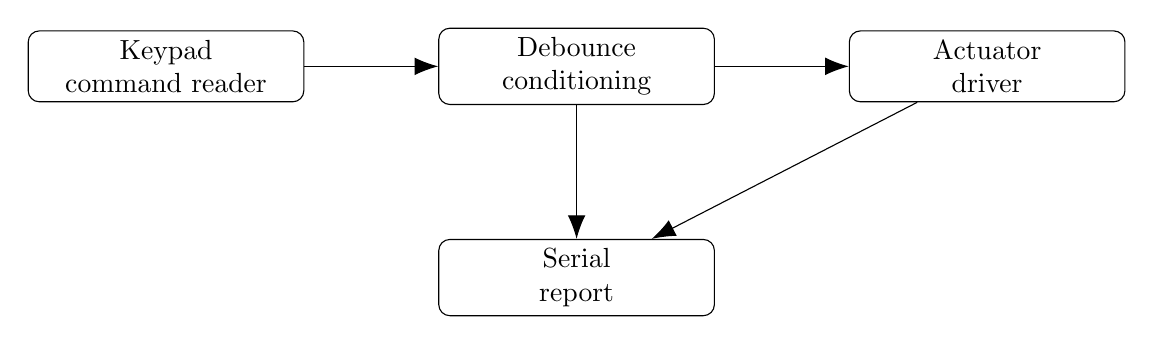
\begin{tikzpicture}[
  node distance=1.7cm,
  block/.style={draw, rounded corners, minimum width=3.5cm, minimum height=0.9cm, align=center},
  arrow/.style={-{Latex[length=3mm]}}
]
\node[block] (keypad) {Keypad\\command reader};
\node[block, right=of keypad] (filter) {Debounce\\conditioning};
\node[block, right=of filter] (drive) {Actuator\\driver};
\node[block, below=of filter] (report) {Serial\\report};
\draw[arrow] (keypad) -- (filter);
\draw[arrow] (filter) -- (drive);
\draw[arrow] (filter) -- (report);
\draw[arrow] (drive) -- (report);
\end{tikzpicture}
\end{center}

\subsection{Task Model}
\begin{itemize}
  \item \textbf{Command task}: scans the keypad every 50 ms and maps \texttt{1/A} to ON and \texttt{0/B} to OFF.
  \item \textbf{Conditioning task}: applies a five-sample temporal debounce filter.
  \item \textbf{Actuator task}: writes the stable state to pin D9 and updates green, red, and yellow LEDs.
  \item \textbf{Report task}: prints raw command, conditioned command, debounce progress, and output state every 500 ms.
\end{itemize}

\section{Implementation}
The implementation is placed in \texttt{src/labs/lab7} and \texttt{include/labs/lab7}. Shared state is protected with a FreeRTOS mutex. The tasks do not access each other's local variables directly; they communicate only through the protected \texttt{Lab7::State} structure.

\begin{lstlisting}
if (sample == output) {
    sameSampleCount = 0;
} else {
    sameSampleCount = (sample == previousSample) ? sameSampleCount + 1 : 1;
    if (sameSampleCount >= StableSamples) {
        output = sample;
        sameSampleCount = 0;
    }
}
\end{lstlisting}

\section{Wokwi Circuit}
The Wokwi diagram is kept identical to the reference implementation for this lab. It uses Arduino Uno, a 4x4 keypad, a relay/LED output on D9, and status LEDs on D10-D12.

\section{Results}
The application compiles for the Arduino Uno PlatformIO environment. During simulation, pressing \texttt{1} or \texttt{A} requests the ON state, while pressing \texttt{0} or \texttt{B} requests the OFF state. The output changes only after the debounce condition is satisfied, which prevents unstable switching.

\section{Conclusion}
The laboratory work demonstrates a robust binary actuator control chain. The functionality is split into acquisition, signal conditioning, output driving, and reporting, matching the requirements for modular embedded actuator applications.

\end{document}
